%!TEX root = ../../super_main.tex

\section{Providing Sensor Data}
\label{sec:providing_sensor_data}

To support this structure of the sensor output, we have designed an abstraction over the different sensors available. This abstraction is designed for concurrent collection of samples, as we want the application to be able to gather information from multiple sources at the same time, meaning that the system is able to, for instance, collect data regarding the motion and location of the participant simultaneously. This is done in order to make sure that the gathered data is obtained according to the desired temporality of the customer, i.e. the time constraints of the campaign as seen in \figref{fig:sample_temporality}.
\\\\
As described in \secref{sec:deriving_the_context_from_sensors}, there exist various types of sensors, each sensing various types of data in various formats. Problems will arise when enforcing temporality of snapshots due to the event oriented nature of sensors in Android. Sensor events will trigger whenever a value is updated. This effectively means that it is impossible to know when these events will trigger. We want to guarantee that measurements can be made with a specific frequency independent on what is supported by the sensor, i.e. measurements can be made more often than what some sensors provide, but also more rarely. For instance the nature of an accelerometer sensor (in Android at least) is that it only raises an event whenever the device is affected in some way, meaning that if the phone is laying completely still this event may never be raised. For sensors of this nature, we need to have some cache that always contains the last measurement of a sensor. 
\\\\
The idea is that this update is completely independent from the the rest of th system, meaning that this update can happen asynchronously. \figref{fig:cache_examples} shows how this independent behavior provides an interface time driven processes that want to acquire the data synchronously. \figref{fig:cache_no_event_between} shows a scenario where some other process request a measurement multiple times where the events from the sensors are not triggered in between. As shown this process will be answered with the same value in both of its requests. However since the underlying sensor have not registered a change the cached measurement must still be correct. Another scenario, as shown in \figref{fig:cache_multiple_event_between}, is that multiple events are triggered between two measurement request from another process. Also here the interface is sound since the value of the sensor that is most recent will be returned, effectively providing the eaves drop interface on event driven sensors we desire.

\begin{figure}[!htbp]
\begin{subfigure}[!t]{.5\textwidth}
  \centering
  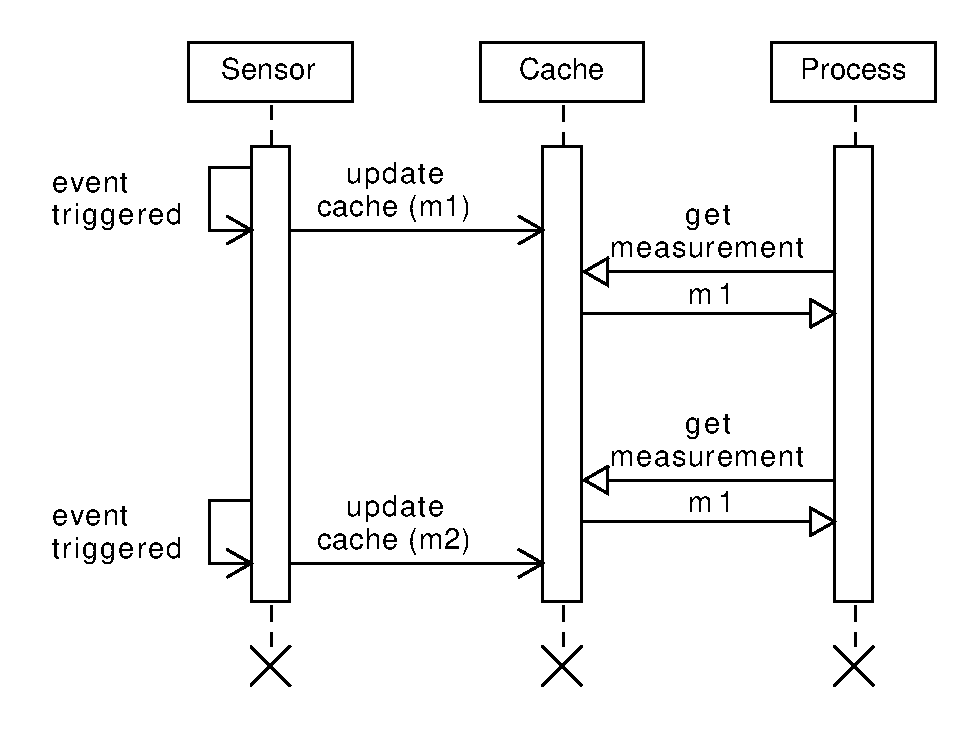
\includegraphics[width=\linewidth]{sensor_providers/cache_example_1}
  \caption{No events between requests.}
  \label{fig:cache_no_event_between}
\end{subfigure}
\begin{subfigure}[!t]{.5\textwidth}
  \centering
  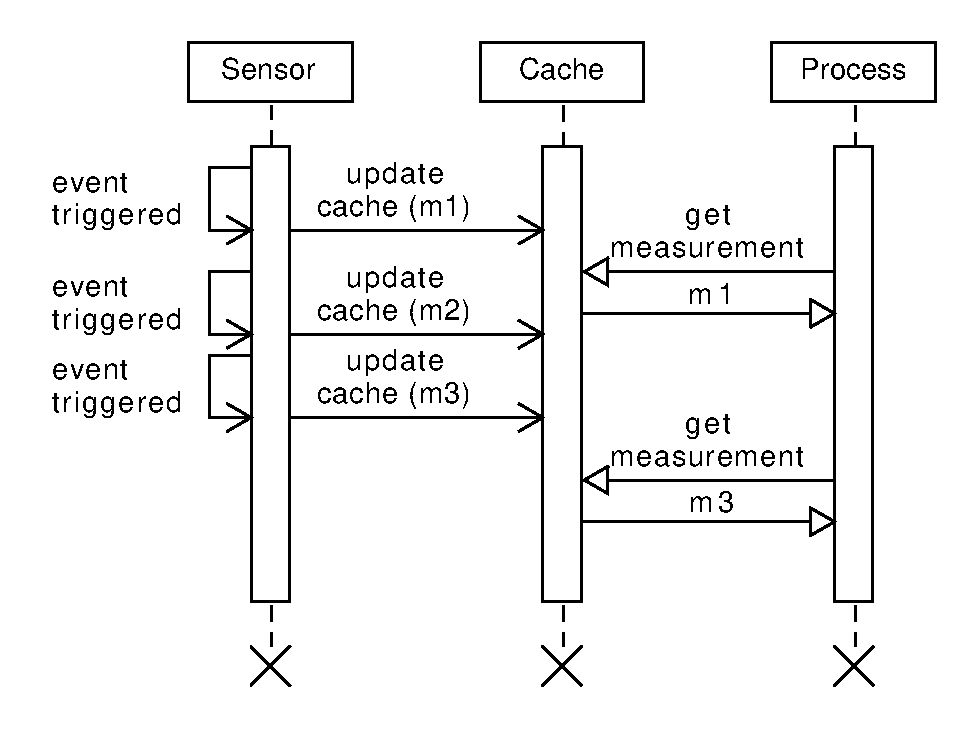
\includegraphics[width=\linewidth]{sensor_providers/cache_example_2}
  \caption{Multiple events between requests.}
  \label{fig:cache_multiple_event_between}
\end{subfigure}
\caption{Measurement caching.}
\label{fig:cache_examples}
\end{figure}
\FloatBarrier

One issue this design might introduce is that we rely on these sensor events to be raised eventually. If this is not the case the cache must contains some default value for a sensor which potentially pollute the sensor measurements until the first event is triggered. This means that until the first event is raised other processes will be answered with some default values. Other type of sensors such as GPS is, as mentioned in \secref{sec:deriving_the_context_from_sensors}, required on demand meaning that we are able to require the GPS location at any given time, meaning that they already provide the behavior that is desired. Some of these on demand sensors might take some time to acquire the information for instance triangulation of satellites for GPS. A potential problem here, in regards to timing, is for this reason latency of which the underlying operating system has before data from this type of sensors are returned to the caller.

\subsection{Sensor Provider}
\label{sub:providing_sensor_data_implementation}
We have implemented an abstract class called \mono{SensorProvider}, which must be specialized for each type of sensor available, both for sensors found in Android, but also for sensors found in the Microsoft Band 2. The abstract class provides functionality that makes it easy to implement specialized implementations for every sensor that we have. Sub-classes of the abstract \mono{SensorProider}, must specify a generic argument, \mono{MeasurementT}, describing the type of measurement that the implementation will make. Besides this, the following methods must also be implemented on the specializations:

% The common interface for these sensor providers is implemented by the following methods:

\begin{description}
	\item[\mono{boolean isSensorAvailable()}] Should return \mono{true} if the sensor is currently available, and ready to take measurements. Should return \mono{false} if the sensor is unavailable or not present on the device.

	\item[\mono{SensorType getSensorType()}] Should return the \mono{SensorType} that the sensor provider implementation will utilize. For instance \mono{SensorType.BAROMETER}.

	\item[\mono{EventListenerRegistrationManager createRegManager()}] Should return an instance of something that implements the \mono{EventListenerRegistrationManager} interface. This interface will enforce the class to implement the following two methods: \mono{void register(int frequency)} and \mono{void unregister()}. These methods will be used by the \mono{SensorProvider} implementation to register the sensor (and its event listeners) when the specific sensor is needed, and unregister them when they are not.

  \item[\mono{FloatTripleMeasurement getDefaultMeasurement()}] Should return an default instance of the \mono{MeasurementT} that the subclass is parameterized with.

\end{description}

Besides implementing these methods, the specializations must also call the \mono{void onNewMeasurement(MeasurementT)}, which will override the cached value, as described in \figref{fig:cache_examples}. With these measurements registered, the \mono{SensorProvider}, and in effect all of the sub-classes, are now able to construct \mono{Sample} objects by reading measurements from the cache with the specific intervals. 
\\\\
All of this effectively means that new sensors can be implemented into the system with very few lines of code. An example of such an implementation can be seen in \lstref{lst:sensor_provider_acclerometer}, which shows how the \mono{AccelerometerSensorProvider} implements and uses the methods described above to make measurements from the phones accelerometer available to our application. The developer have to write relative few lines of code to enable this provider for a any new type of sensor. To do so the developer must, as seen in \lineref{line:sensor_provider_extends}, subclass the \mono{Sensorprovider} with the generic parameter \mono{FloatTripleMeasurement} which is the type of measurement the accelerometer produces. Furthermore he have to override the abstract methods as follows: \linesref{line:isSensorAvailable_start}{line:isSensorAvailable_end} for the \mono{isSensorAvailable}, \lineref{line:getSensorType} for \mono{getSensorType}, \lineref{line:createRegManager} and \linesref{line:createRegManager_start}{line:createRegManager_end} for \mono{createRegManager} and lastly \lineref{line:getDefaultMeasurement} for \mono{getDefaultMeasurement}.

\lstinputlisting[
   style = Java,
   caption = {Implementation of sensor provider for Accelerometer.},
   label = {lst:sensor_provider_acclerometer},
   float,
]{content/gathering_sensor_data/code_snippets/sensor_provider_acclerometer.java}

% The abstract \mono{isSensorAvailable()} method allows the subclasses of \mono{SensorProvider} a way of specifically checking if the device has that sensor available. This might for example be useful in order to determine which campaigns should be available to which participants at some point, or detecting if a wearable device has been disconnected. \mono{retrieveSampleForDuration()} is a method that every subclass has to implement, which specifies how a sample is created for this specific sensor. The \mono{retrieveSamplesForDuration()} method is implemented on the \mono{SensorProvider} class, i.e. not abstract like the other two methods, and is the method that makes all the different providers work asynchronously. The method returns a \mono{Future<List<Sample>{}>}. A future, in Android, is the result of an asynchronous computation. The result from a future can be retrieved by calling the \mono{get()} method on the future object, which is a blocking call. Android then provides different methods to check whether or not the computation is completed, in progress, and so on. The method works by submitting a \mono{Callable} to a thread pool, which will eventually return a list of samples, i.e. the future. This callable contains a \mono{TimerTask}, which is a task that is repeated a certain amount of times, that in return calls the \mono{retrieveSampleForDuration()} method. In that way, we have a \mono{Callable} which at some point returns the desired amount of samples. 
% \\\\
% The \mono{retrieveSampleForDuration()} method has, in all the subclasses of \mono{SensorProvider}, been implemented by using a native method called \mono{onSensorChanged()}. As the name implies, this event is triggered whenever a sensor changes its state. This is a potential issue, since not all sensors provide continuous data, and not all sensors will change in the time limit that is allowed between two measurements (see \figref{fig:sample_temporality}). A potential solution to this is to always store the previous state, and if the event is not triggered within the alloted time, simply use the cached value. 
% \\\\
% Another potential issue with this implementation is the desire for asynchronism, which we implemented by using \mono{future} objects. Since we cannot know for certain when different asynchronous calls are finished, it might become difficult to create a snapshot and send it to the database.

% \lstinputlisting[
%    style = java,
%    caption = {Property similarity on a component.},
%    label = {lst:attribute_difference},
%    float,
%]{content/implementation/annotation/attribute_difference.java}